%%%%%%%%%%%%%%%%%%%%%%%%%%%%%%%%%%%%%%%%%%%%%%%%%%
% Basic setup. Most papers should leave these options alone.
\documentclass[a4paper,fleqn,usenatbib]{mnras}

% MNRAS is set in Times font. If you don't have this installed (most LaTeX
% installations will be fine) or prefer the old Computer Modern fonts, comment
% out the following line
\usepackage{newtxtext,newtxmath}
% Depending on your LaTeX fonts installation, you might get better results with one of these:
%\usepackage{mathptmx}
%\usepackage{txfonts}

% Use vector fonts, so it zooms properly in on-screen viewing software
% Don't change these lines unless you know what you are doing
\usepackage[T1]{fontenc}
\usepackage{ae,aecompl}


%%%%% AUTHORS - PLACE YOUR OWN PACKAGES HERE %%%%%

% Only include extra packages if you really need them. Common packages are:
\usepackage{graphicx}	% Including figure files
\usepackage{amsmath}	% Advanced maths commands
\usepackage{amssymb}	% Extra maths symbols
\usepackage{tikz}
\DeclareMathAlphabet{\mathcal}{OMS}{cmsy}{m}{n}
\usetikzlibrary{bayesnet}
%%%%%%%%%%%%%%%%%%%%%%%%%%%%%%%%%%%%%%%%%%%%%%%%%%

%%%%% AUTHORS - PLACE YOUR OWN COMMANDS HERE %%%%%

% Please keep new commands to a minimum, and use \newcommand not \def to avoid
% overwriting existing commands. Example:
%\newcommand{\pcm}{\,cm$^{-2}$}	% per cm-squared
\newcommand{\name}{Steve-o}
\newcommand{\myemail}{samuelreay@gmail.com}
\newcommand\abs[1]{\left|#1\right|}
\newcommand {\etal} {\emph{~et~al.} }
\newcommand{\green}{\color{green}}
\newcommand{\blue}{\color{blue}}
\newcommand{\red}{\color{red}}

\newcommand{\kmsmpc}{{\rm km}\,{\rm s}^{-1}\,{\rm Mpc}^{-1}}
\newcommand{\cov}{\mathcal{C}}
\newcommand{\Z}{\mathcal{Z}}

\defcitealias{Guy2010}{G10}
\defcitealias{Chotard2011}{C11}
\defcitealias{Rubin2015}{R15}	
\defcitealias{Scolnic2016}{SK16}	 
\newcommand{\gten}{\citetalias{Guy2010}}
\newcommand{\celeven}{\citetalias{Chotard2011}}
\newcommand{\rubin}{\citetalias{Rubin2015}}
\newcommand{\sk}{\citetalias{Scolnic2016}}
\newcommand{\angstrom}{\mbox{\normalfont\AA}}


\graphicspath{ {./figures/} }
%%%%%%%%%%%%%%%%%%%%%%%%%%%%%%%%%%%%%%%%%%%%%%%%%%

%%%%%%%%%%%%%%%%%%% TITLE PAGE %%%%%%%%%%%%%%%%%%%

% Title of the paper, and the short title which is used in the headers.
% Keep the title short and informative.
\title[\name]{\name: A hierarchical Bayesian model for Supernova Cosmology}

% The list of authors, and the short list which is used in the headers.
% If you need two or more lines of authors, add an extra line using \newauthor
\author[S. R. Hinton et al.]{
	Samuel R. Hinton,$^{1,2}$\thanks{E-mail: samuelreay@gmail.com}
	Alex G. Kim,$^{3}$
	Tamara M. Davis$^{1,2}$
	\\
	% List of institutions
	$^{1}$School of Mathematics and Physics, The University of Queensland, Brisbane, QLD 4072, Australia\\
	$^{2}$ARC Centre of Excellence for All-sky Astrophysics (CAASTRO)\\
	$^{3}$Physics Division, Lawrence Berkeley National Laboratory, 1 Cyclotron Road, Berkeley, CA 94720, USA
}

% These dates will be filled out by the publisher
\date{Accepted XXX. Received YYY; in original form ZZZ}

% Enter the current year, for the copyright statements etc.
\pubyear{2017}

% Don't change these lines
\begin{document}
\label{firstpage}
\pagerange{\pageref{firstpage}--\pageref{lastpage}}
\maketitle











% Abstract of the paper
\begin{abstract}
We present a hierarchical Bayesian model for use in supernova cosmology which takes into account full analysis systematics, Malmquist bias, underlying populations and standardisation coefficients. Our model is optimised for efficient fitting and has been validated on a combined dataset of more than $250\,000$ supernovae. Simplified statistical simulations for ideal supernovae cosmology show no bias, and sophisticated SNANA simulations quantify the bias for Flat $w$CDM with a matter prior $\Omega_m \sim \mathcal{N}(0.3, 0.01)$ allow rigorous determination of model bias in $w$ when provided with information on matter density (such as might be found from CMB constraints). Bias is found to range from $-0.15\sigma$ to $+0.27\sigma$ across intrinsic dispersion models for datasets of comparable strength to the Dark Energy Survey three-year analysis. 
\end{abstract}

% Select between one and six entries from the list of approved keywords.
% Don't make up new ones.
\begin{keywords}
keyword1 -- keyword2 -- keyword3
\end{keywords}









%%%%%%%%%%%%%%%%% BODY OF PAPER %%%%%%%%%%%%%%%%%%

\section{Introduction}

Almost two decades have passed since the discovery of the accelerating universe \citep{Riess1998, Perlmutter1999}. Since that time, of the number of observed Type Ia supernovae (SN Ia) have increased by more than an order of magnitude thanks to modern surveys at both low redshift \citep{Bailey2008, Freedman2009, Hicken2009,  Contreras2010, Conley2011}, and higher redshift \citep{Astier2006, Wood-Vasey2007, Balland2009, Amanullah2010}. Cosmological analysis of these supernova samples \citep{Kowalski2008, Conley2011, Suzuki2012, Betoule2014, Rest2014} have been combined with complimentary probes of large scale structure \citep{Alam2017} and the CMB \citep{Hinshaw2013, PlanckCollaboration2013}, and yet, despite these prodigious efforts, the nature of dark energy remains an unsolved mystery.

In attempts to tease out the nature of dark energy, currently running and planned surveys are once again ramping up their statistical power. The Dark Energy Survey \citep[DES,][]{Bernstein2012, Abbott2016} will be observing thousands of Type Ia supernova, attaining both spectroscopic and photometric confirmation. The Large Synoptic Survey Telescope \citep[LSST,][]{Ivezic2008, LSSTScienceCollaboration2009} will produce scores of thousands of photometrically classified supernovae. Such increased statistical power demands a similarly increased fidelity and flexibility in modelling the supernovae for cosmological purposes, as systematic uncertainty will prove to be the limiting factor in our analyses.

As such, staggering effort is being put into developing more sophisticated supernovae analyses. First used in ESSENSE analyses \citep{Wood-Vasey2007}, and then refined and improved in \citet{Kessler2009}, the role of simulations has become increasingly important in determining biases and validating models. \citet{Betoule2014} make use of redshift dependent $\mu$-bias to correct their analyses, and more recently \citet{Scolnic2016} and \citet{Kessler2017} explore simulation corrections as a function of redshift, stretch and colour to better remove fitting biases. Approximate Bayesian computation methods also make use of simulations, trading traditional likelihoods and analytic approximations for more robust models with only the cost of increased computational time \citep{Weyant2013, Jennings2016}. Hierarchical Bayesian Models abound \citep{Mandel2009, March2011, March2014, Rubin2015, Shariff2016, Roberts2017}, however often face difficulties finding sufficient analytic approximations for complicated effects such as Malmquist bias.


In this paper, we lay out a new hierarchical model that advances the past work of \citet{Rubin2015} to include more robust treatment of systematics and selection effects whilst improving computational performance. Section \ref{sec:review} is dedicated to a quick review of the supernovae cosmology. In Section \ref{sec:method} we outline our methodology. Model verification on simulated datasets is given in Section \ref{sec:verification}, along with details on potential areas of improvement.









\section{Review}
\label{sec:review}

Whilst supernova observations take the form of time-series photometric measurements of brightness in many photometric bands, most analyses do not work from these measurements of apparent magnitude and colour. Instead, most techniques fit these observations of magnitude (along with redshift) to a supernova model, with the most widely used being that of the empirical SALT2 model \citep{Guy2007, Guy2010}. This model is trained separately before fitting the supernovae light curves for the cosmology selected supernova sample \citep{Guy2010, Mosher2014}. The resulting output from the model is, for each supernova, a characterised amplitude $x_0$ (which can be converted into apparent magnitude $m_B = -2.5\log(x_0)$), a stretch term $x_1$ and colour term $c$, along with a covariance matrix describing the uncertainty on these summary statistics. As such, the product at the end is a (redshift-dependent) population of $m_B$, $x_1$ and $c$.

The underlying actual supernova population is not as clear cut, and indeed accurately characterising this population, its evolution over redshift and effects from environment is one of the challenges of supernova cosmology. However, given some modelled underlying population that lives in the redshift-dependent space $M_B$, $x_1$ and $c$, the introduction of cosmology into the model is simple -- it is encoded in the functional map between those two populations, from apparent magnitude space to absolute magnitude. Specifically, for any given supernova our functional map may take the traditional form:
\begin{equation}
M_B = m_B + \alpha x_1 - \beta c - \mu(z) + \text{corrections},
\end{equation}
where $\alpha$ is the stretch correction \citep{Phillips1993}, and $\beta$ is the colour correction \citep{Tripp1998} that respectively encapsulate the empirical relation that broader and bluer supernovae are brighter. The $\text{corrections}$ term at the end often includes corrections for host galaxy environment, as this has statistically significant effects on supernova properties \citep{Kelly2010, Lampeitl2010, Sullivan2010, DAndrea2011, Gupta2011, Johansson2013, Rigault2013, Uddin2017}. The cosmological term, $\mu(z)$ represents the distance modulus, and is precisely known given cosmological parameters and an input redshift.

\subsection{Traditional Analyses}

Traditional $\chi^2$ analyses such as that found in \citet{Kowalski2008, Conley2011, Betoule2014}, minimise the difference in distance modulus between the cosmologically predicted values $\mu_C$ and the observed distance modulus $\mu_{\rm obs}$, shown respectively below:
\begin{align}
\mu_C &= 5 \log\left[ \frac{(1+z)r}{10} \right]\\
r& =\frac{c}{H_0} \int_0^z \frac{dz'}{\sqrt{ \Omega_m (1+z')^3 + \Omega_k (1 + z')^2 + \Omega_\Lambda (1+z')^{3(1+w)}}} \label{eq:mu0}\\
\mu_{\rm obs} &= m_B + \alpha x_1 - \beta c - M_B \label{eq:mu1}
\end{align}
The minimising function is then given as
\begin{equation}
\chi^2 = (\mu_{\rm obs} - \mu_C)^\dagger C^{-1} (\mu_{\rm obs} - \mu_C)
\end{equation}
where $C^{-1}$ is an uncertainty matrix that combines the uncertainty from the SALT2 fits, intrinsic dispersion, calibration, dust, peculiar velocity and many other factors (see \citet{Betoule2014} for a review). The benefit this analysis methodology provides is speed - for samples of hundreds of supernovae, efficient matrix inversion algorithms allow the likelihood to be evaluated quickly. The speed comes with two costs. Firstly, formulating a $\chi^2$ likelihood requires a loss of model flexibility by building into the model assumptions of uncertainty Gaussianity. Secondly, the computational efficiency is dependent on inverting a covariance matrix with dimensionality linearly proportional to the number of supernovae. As this number increases, the cost of inversion rises quickly, and is not viable for samples with thousands of supernovae.

Selection efficiency, such as the well known Malmquist bias \citep{MalmquistK.G.1922} is accounted for by correcting data. Simulations following survey observational strategies and geometry are used to calculate the expected bias in distance modulus, which is then added onto the observational data. As these effects are not built into the likelihood, their influence on the error budget is not captured fully in the $\chi^2$ distribution, and any subtle correlations between cosmological or population parameters and the bias is lost.

\subsection{Approximate Bayesian Computation}

To try and escape the limitations of the traditional analysis methodology, several recent methods have adopted Approximate Bayesian Computation, where supernova samples are forward modelled in parameter space and compared to observed distributions. \citet{Weyant2013} provides an introduction into ABC methods for supernova cosmology in the context of the SDSS-II results \citep{Sako2014} and Flat $\Lambda$CDM cosmology, whilst \citet{Jennings2016} demonstrates their \textit{superABC} method on simulated first season Dark Energy Survey samples, described in \citet{Kessler2015}. In both examples, the supernova simulation package SNANA \citep{Kessler2009a} is used to forward model the data at each point in parameter space.

By building the systematic uncertainties and selection effects into the simulation package, there is vastly more freedom in how to treat and model those effects. Data does not need to be corrected, analytic approximations do not need to be applied, we are free to incorporate algorithms that simply cannot be expressed in a tractable likelihood. This freedom comes with a cost -- computation. The classical $\chi^2$ method's most computationally expensive step in a fit is matrix inversion. For ABC methods, we must instead simulate an entire supernova population in its entirety -- drawing from underlying supernova populations, modelling light curves, applying selection effects, fitting light curves and applying data cuts. This is an intensive process. Luckily, efficient sampling algorithms that have walkers that rely on the Markov properties of groups instead of individual walkers, such as Ensemble sampling \citep{Foreman-Mackey2013} allow easy parallelisation of parameter fits and can help ease the computational burden.

One final benefit of ABC methods is that they can move past the traditional treatment of supernovae with summary statistics ($m_B$, $x_1$ and $c$). \citet{Jennings2016} presents both a metric used to compare forward modelled summary statistic populations (denoted the `Tripp' metric) and a metric directly applicable to the observed supernova light curves themselves, however evaluation of systematic uncertainty was only performed using the Tripp metric.

\subsection{Hierarchical Bayesian Models}

Sitting comfortably between the traditional models simplicity and the complexity of forward modelling lies Hierarchical Bayesian Models. With the introduction of multiple layers in our model, we can add far more flexibility than a traditional analysis whilst still maintaining most of the computational benefits that come from having a tractable likelihood. \citet{Mandel2009}, \citet{Mandel2011} and \citet{Mandel2017} construct a hierarchical model that they apply to the light curve fitting for supernova. \citet{March2011} derive a hierarchical model and simplify it by analytically marginalising over nuisance parameters to provide a model that offers increased flexibility with reduced uncertainty over the traditional method, but does not incorporate bias correction. \citet{March2014, Karpenka2015} improve upon this by incorporating redshift-dependent magnitude corrections from \citet{Perrett2010} to remove bias, and validate on 100 realisations of SNLS like simulations. The recent BAHAMAS model \citep{Shariff2016} builds off this and reanalyses the JLA dataset (using their redshift dependent bias corrections), whilst including extra freedom in the correction factors $\alpha$ and $\beta$, finding evidence for redshift dependence on $\beta$. \citet{Ma2016} also performed a reanalysis of the JLA dataset, finding significant differences in $\alpha$ and $\beta$ values from the original as well by correctly including in their likelihood the determinant of the global covariance matrix. Notably, these methods rely on data that is bias corrected or ignore biases, however the UNITY framework given by \citet{Rubin2015} incorporates selection efficiency analytically in the model, and is applied to the Union 2.1 dataset \citep{Suzuki2012}. The simplification made by the UNITY analysis is that the bias is well described by an analytic function, and this function is fixed such that selection effects are assumed to be determined with perfect precision. Their model was validated on thirty realisations of statistics. Whilst there are a large amount of hierarchical models available, all sofar mentioned, in the case where any validation has been done, have been done on either $\Lambda$CDM cosmology or Flat $\Lambda$CDM cosmology. None of them have undergone high-statistics simulation verification for $w$CDM cosmology to quantify each models respective bias, which is becoming critically important as precision supernovae cosmology comes into its own and focus shifts from determination of $\Omega_m$ to $w$.

The well known BEAMS (Bayesian estimation applied to multiple species) methodology from \citet{Kunz2007} has been extended and applied in several works \citep{Hlozek2012}, mostly lately to include redshift uncertainty for photometric redshift application as zBEAMS \citep{Roberts2017} and to include simulated bias corrections in \citet{Kessler2017}. For the latter case, by inferring biases using Bayesian models, sophisticated corrections can be calculated and then applied to more traditional $\chi^2$ models.

The flexibility afforded by a hierarchical model allows for investigations into different treatments of underlying supernova magnitude, colour and stretch populations, supernovae type rates and redshift distributions, host-galaxy corrections and redshift evolution, each of which will be discussed further in the outline of our model below.









\section{Our Method}
\label{sec:method}

We construct our Bayesian Hierarchical Model with several goals in mind: creation of a redshift-dependent correlated underlying supernova population, increased treatment of systematics, and analytic correction of selection effects. As this is closest to the UNITY method from \citet[][hereafter denoted \rubin]{Rubin2015}, we follow a similar model scaffold, and construct the model in Stan \citep{Carpenter2017, StanDevelopmentTeam2017} which uses automatic differentiation and the no-U-turn Sampler (NUTS), which is a variant of Hamiltonian Monte Carlo, to efficiently sample high dimensional parameter space.

At the most fundamental level, a supernova analysis is simply a mapping from an underlying population onto an observed population, where cosmology is encoded directly in the mapping function. The difficulty arises both in adequately describing the biases in the mapping function, and in adding sufficient, physically motivated flexibility in both of these populations whilst not adding \textit{too} much flexibility, such that model fitting becomes pathological due to increasing parameter degeneracies within the model.


\subsection{Observables Nature Provides: Populations}

Like most of the BHM methods introduced previously, we work from the summary statistics as well, where each observed supernova has an apparent magnitude $\hat{m_B}$, stretch $\hat{x_1}$ and colour $\hat{c}$, with uncertainty $\cov$ on those values. Additionally, each supernova has an observed redshift $\hat{z}$ and a host galaxy mass associated with it, $\hat{m}$, where the mass measurement takes the form of a probability of being above $10^10$ solar masses. Given machine learning classifiers to type supernovae, we will also have a probability of being a Type Ia, $\hat{p}$. Our set of observables is therefore given as $\lbrace \hat{m_B}, \hat{x_1}, \hat{c}, \hat{z}, \hat{p}, \hat{m}, \cov \rbrace$, as shown in the probabilistic graphical model (PGM) in Figure \ref{fig:pgm}.

The first layer of the hierarchy represents the latent population of $m_B$, $x_1$ and $c$. This can be thought of as the `true' values for the supernova, and with correct summary statistics and uncertainty would be normally distributed around the observed values such that 
\begin{equation}
P(\hat{m_B},\hat{x_1},\hat{c}|m_B, x_1, c,\cov) = \mathcal{N}(\lbrace \hat{m_B},\hat{x_1},\hat{c} \rbrace|\lbrace m_B, x_1, c \rbrace, \cov). \label{eq:pop}
\end{equation}
However, the presence of chromatic smearing in the intrinsic supernova population \citep{Guy2010, Chotard2011} means the summary statistics report from light curve fitting are not Gaussian. We model the extra dispersion included in the observations from colour smearing by adding extra independent uncertainty on the colour observation. As shown in \citep{Kessler2013}, the extra dispersion shows heavy redshift dependence. As this may represent underlying physics more than the effects of Malmquist bias, we decide to incorporate redshift dependence in our extra uncertainty. We thus add $\kappa_0 + \kappa_1 z$ to our observed colour uncertainty (in quadrature), where $\kappa_0$ and $\kappa_1$ are subject to strong Cauchy priors centered on zero and with width $0.002$, to enforce minimum possible extra uncertainty in our model. Each survey has its own set of $\kappa$ parameters. Furthermore, we use fiducial simulations (discussed further in Section \ref{sec:selection}) to characterise the bias in the mean colour measured as a function of redshift, and subtract this bias from our observed data. We allow the amount of bias to be parametrised to account for different intrinsic scatter models, where parameter $s_c$ controlled the fraction of bias subtraction - 0 for no bias, up to 1 for the maximum bias found in simulations (which corresponded to the intrinsic scatter model from \citet{Chotard2011}). Unlike $\kappa_0$ and $\kappa_1$, which are redefined for each survey, $s_c$ represents a universal shift in supernovae biases. We place a uniform prior on $s_c$.

As we are focused on the spectroscopically confirmed supernovae for this iteration of the method, we assume the observed redshift $\hat{z}$ is the true redshift $z$ such that $P(\hat{z}|z) = \delta(\hat{z} - z)$. Similarly, we take the mass probability estimate $\hat{m}$ as correct, and do not model a latent variable.

\begin{figure}
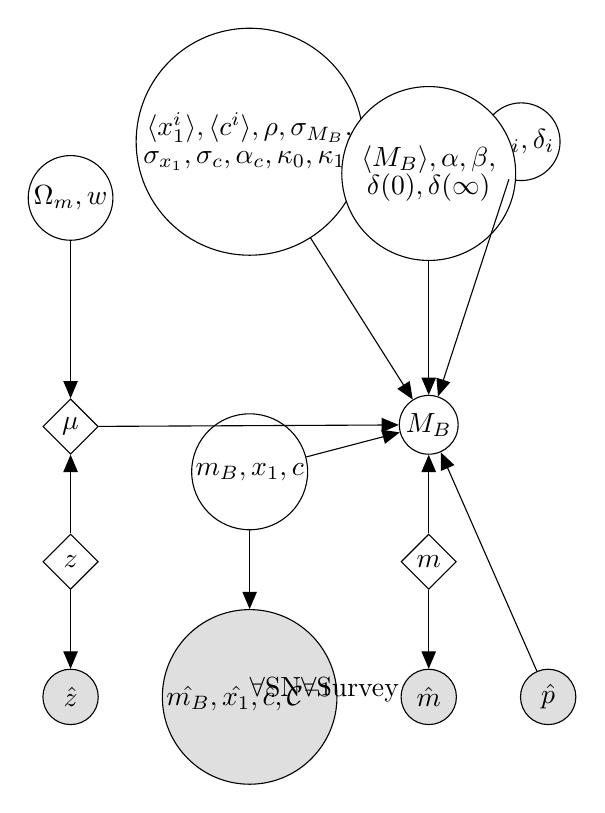
\begin{tikzpicture}
% Obs nodes
\node[obs]  (obssum) {$\hat{m_B}, \hat{x_1}, \hat{c}, \mathcal{C}^{-1}$};
\node[obs, left=0.8cm of obssum]  (zobs) {$\hat{z}$};
\node[obs, right=0.8cm of obssum]  (mobs) {$\hat{m}$};
\node[obs, right=0.8cm of mobs]  (pobs) {$\hat{p}$};

% Latent nodes
\node[latent, above=of obssum] (sum) {$m_B, x_1, c$};
\node[det, above=of zobs] (z) {$z$};
\node[det, above=of mobs] (m) {$m$};
\node[det, above=of z] (mu) {$\mu$};
\node[latent, above=of m] (MBobs) {$M_B$};
% Survey nodes
\node[latent, above=of sum, yshift=1cm,text width=2.7cm, align=center] (pop1) {$\langle x_1^i \rangle, \langle c^i \rangle,\rho,\sigma_{M_B}, $\\$ \sigma_{x_1}, \sigma_c, \alpha_c, \kappa_0, \kappa_1, s_c$ };
\node[latent, right=1.5cm of pop1, align=center] (sf) {$\Delta_i, \delta_i$};
% Global nodes
\node[latent, above=2cm of mu]  (cosmo) {$\Omega_m, w$};
\node[latent, above=1.7cm of MBobs, text width=2cm, align=center]  (ab) {$\langle M_B \rangle, \alpha, \beta,$\\$\delta(0), \delta(\infty)$};

% Connect the nodes
\edge {sum} {obssum};
\edge {z} {zobs};
\edge {m} {mobs};
\edge {z,cosmo} {mu};
\edge {mu, sum, m, pop1, ab, pobs, sf} {MBobs};

% Plates
\plated[thick] {sn} {(obssum)(zobs)(mobs)(pobs)(sum)(z)(m)(mu)} {$\forall\ \rm{SN}$} ;
\plated[thick] {survey} {(sn)(pop1)} {\\$\forall\ \rm{Survey}$} ;
\end{tikzpicture}
\caption{Probabilistic graphical model for our likelihood. Double-lined nodes represent observed variables, diamond nodes represent deterministic variables, and standard nodes represent fit variables.}
\label{fig:pgm}
\end{figure}


\subsection{Underlying Population}

The underlying supernova population is often treated with two components - a population distribution in colour and stretch, and intrinsic dispersion. Analytic models often treat the colour and stretch populations with a skew normal and normal, respectively, and have them as independent. Intrinsic dispersion is treated in a variety of manners in other models, from representing it simply as (Gaussian) scatter on the absolute magnitude of the supernova population, to correlated multivariate normal scatter on the combined magnitude, stretch and colour distribution. Additionally, redshift drift of populations' mean colour and stretch will introduce a cosmological bias in our fits unless the population possesses similar ability to change as a function of redshift. 

We follow prior work and model the colour population as an independent redshift-dependent skew normal for each survey. For the stretch population, we adopt a redshift-dependent normal, and magnitude dispersion is modelled as a normal. Following {\rubin} we allow the mean colour and stretch to vary over redshift, anchoring four equally spaced redshift nodes spanning the redshift range of each survey, linearly interpolating between the nodes. These nodes are represented as $\langle x_1^i \rangle$ and $\langle c^i \rangle$. Both the colour and stretch means are modelled with normal priors. Initial versions of our model adopted a fully covariant multivariate skew normal (with skewness set to zero only for the magnitude component), however pathological fitting complications required us to simplify our treatment. We parameterise the standard skew normal skewness $\alpha_c$ by sampling $\delta_c = \alpha_c / \sqrt{1 + \alpha_c^2}$ which itself is given a uniform prior $\mathcal{U}(0,0.98)$. The width of the population, represented by the vector $\lbrace \sigma_{M_B}, \sigma_{x_1}, \sigma_c \rbrace$ is subject to Cauchy priors, however are sampled in log space for efficiency in sampling close to zero. 

As such, the only constant between survey populations is the absolute magnitude $M_B$, with the skewness, redshift-dependent means and width fit individually for each survey. The probability for a supernova to have true values $M_B$, $x_1$, $c$ given the underlying population is thus given as
\begin{align}
P(M_B, x_1, c, z | \langle M_B \rangle, \langle x_1(z) \rangle, \langle c(z) \rangle, \rho, \sigma_{m_B}, \sigma_{x_1}, \sigma_c, \alpha_c) = \notag \\
\mathcal{N}(M_B|\langle M_B \rangle, \sigma_{M_B}) \mathcal{N}(x_1 | \langle x_1(z) \rangle \sigma_{x_1}) \mathcal{N}^{\rm{skew}}(c| \langle c(z) \rangle, \sigma_c, \alpha_c) \label{eq:l1}.
\end{align}


On top of the Ia populations, as described above, we also include a simplistic outlier population that also follows {\rubin} \citep[and therefore ][]{Kunz2007} as a Gaussian mixture; where the mean of the population is fixed to the Ia population, but the population width is set to a width of $\sigma^{\rm outl} = 1$ in $M_B$, $x_1$ and $c$. With the spectroscopic DES sample, the contamination rate is expected to be far too low to actually fit contamination population, however in future works with photometric samples that will suffer from significantly more contamination it will be required that extra degrees of freedom are afforded the outlier population. Proof of concept simulation fits show that an acceptable parametrisation is to represent the typically brighter contaminant population as $\langle M_B^{\rm outl} \rangle = \langle M_B \rangle - \delta_{M_B}^{\rm outl}$, where $\delta_{M_B}^{\rm outl}$ is constrained to be positive, or even to be greater than a small positive number to reduce degeneracy between the two populations. For the purposes of the DES spectroscopic sample, which will be dominated by confirmed Type Ia supernovae, $\delta_{M_B}^{\rm outl} =0$. We assume that supernovae fall into either population as determined by their observed classification probability $\hat{p}$.


\subsection{Population Map}

\subsubsection{Cosmology}

We formulate our model with three different cosmological parameterisations; Flat $\Lambda$CDM, Flat $w$CDM and standard $\Lambda$CDM. $\Omega_m$ is given the prior $\mathcal{U}(0.05, 0.99)$, $\Omega_\Lambda$ was treated with $\mathcal{U}(0, 1.5)$ and the equation of state $w$ was similarly set to a flat prior $\mathcal{U}(-0.4, -2.0)$. For calculating the distance modulus, we fix $H_0 = 70 \kmsmpc $. 

\subsubsection{Standardisation Parameters}

With increasingly large datasets and more nuanced analyses, the choice of how to handle $\alpha$ and $\beta$ becomes an important consideration when constructing a model. {\rubin} employs a broken linear relationship for both colour and stretch, where different values of $\alpha$ and $\beta$ are adopted depending on whether $x_1$ and $c$ are respectively positive or negative (although the cut could be placed at a location other than 0). \citet{Shariff2016} instead of employ a colour-dependent $\beta$, model $\beta$ as redshift-dependent, testing two phenomenological models; $\beta(z) = \beta_0 + \beta_1 z$ and $\beta(z) = \beta_0 + \Delta \beta\left(0.5 + \arctan(100(z - z_t)) / \pi\right)$, where the later effects a rapid but smooth change in $\beta$ at a turnover redshift $z_t$.

We tested two models against simulated supernova sets; $\beta(c) = \beta_0 + \beta_1 c$ and $\beta(z) = \beta_0 + \beta_1 z$. See Section \ref{sec:simdes} for details on simulation generation. We found for both models that non-zero values for $\beta_1$ are preferred (even with constant $\beta$ used in simulation) due to severe degeneracy with selection effects. This degeneracy resulted in a significant bias in recovered cosmology, and so in our final model we continue to adopt the constant $\alpha$ and $\beta$ found in traditional analyses. As such, our calculation of distance modulus $\mu$ mirrors that found in Equations \eqref{eq:mu0} and \eqref{eq:mu1}.

\subsubsection{Host Galaxy Environment}

It is now well known that host galaxy environment has a significant effect on supernova properties. The latest sample of over 1300 spectroscopically confirmed Type Ia supernovae show $>5\sigma$ evidence for correlation between host mass and luminosity \citep{Uddin2017}. The traditional correction, as employed in analyses such as \citet{Suzuki2012} and \citet{Betoule2014} invoke a step function such that $\Delta M = 0.08 \mathcal{H}(\log(M) - 10))$, where $\mathcal{H}$ is the Heaviside step function and $M$ is the galaxy mass in solar masses. The scale of this step function varies from analysis to analysis, with the 0.08 value shown previously sourced from \cite{Sullivan2010} and used in \citet{Betoule2014}. In this work we adopt the model used in {\rubin}, which follows the work from \citet{Rigault2013}, such that we introduce two parameters to incorporate a redshift-dependent host galaxy mass correction:
\begin{equation}
\Delta M = \delta(0) \left[ \frac{1.9\left(1 - \frac{\delta(0)}{\delta(\infty)}\right)  }{0.9 + 10^{0.95z}} + \frac{\delta(0)}{\delta(\infty)}\right]
\end{equation}
We also take flat priors on the parametrisation $\delta(0)$, $\delta(0)/\delta(\infty)$. With this correction, our calculation of absolute magnitude becomes
\begin{align}
M_B = m_B - \mu(z) - \alpha x_1 + \beta c - \Delta M \cdot m. \label{eq:l2}
\end{align}



\subsubsection{Uncertainty Propagation}
\label{sec:systreat}
The chief difficulty with including systematic uncertainties in supernova analyses is that they generally occur during the observational pipeline, and have difficult-to-model effects on the output observations. As such, the normal treatment for systematics is to compute their effect on the supernova summary statistics -- computing the numerical derivatives $\frac{\partial \hat{m_B}}{\partial \Z_i}$, $\frac{\partial \hat{x_1}}{\partial \Z_i}$, $\frac{\partial \hat{c}}{\partial \Z_i}$, where $\Z_i$ represents the $i$\textsuperscript{th} systematic.

Assuming that the gradients can be linearly extrapolated -- which is a reasonable approximation for modern surveys with high quality control of systematics -- we can incorporate into our model a deviation from the observed original values by constructing a $(3 \times N_{\rm sys})$ matrix containing the numerical derivatives for the $N_{\rm sys}$ systematics and multiplying it with the row vector containing the offset for each systematic. By scaling the gradient matrix to represent the shift over $1\sigma$ of systematic uncertainty, we can simply enforce a unit normal prior on the systematic row vector to increase computational efficiency.

This method of adjusting the observed summary statistics is used throughout the traditional and BHM analyses, however it is normally constrained to band systematics. That is, each band for each survey has two systematics associated with it - the calibration uncertainty and the filter wavelength uncertainty. We include these in our approach, in addition to including HST Calspec calibration uncertainty, 10 SALT2 model systematic uncertainties, a dust systematic, a global redshift bias systematic and also the systematic peculiar velocity uncertainty. This gives thirteen global systematics shared by all surveys, plus two systematics per band in each survey. Denoting $\eta \equiv \lbrace m_B, x_1, c \rbrace$, our initial conditional likelihood for our observed summary statistics shown in Equation \eqref{eq:pop} becomes
\begin{align}
P\left(\hat{\eta}, \frac{\partial \hat{\eta}}{\partial \Z_i} | \eta, \delta \Z_i, C\right) = \mathcal{N}\left(\hat{\eta} + \delta \Z_i \frac{\partial \hat{\eta}}{\partial \Z_i}|\eta,\cov\right). \label{eq:l3}
\end{align}



\subsubsection{Selection Effects}
\label{sec:selection}
Our treatment of selection effects is to incorporate selection efficiency into our model, rather than relying on simulation-driven data corrections. As such, we need to describe the probability that the events we observe are both drawn from the distribution predicted by the underlying theoretical model \textit{and} that those events, given they happened, are subsequently successfully observed.  To make this extra conditional explicit, we can write the likelihood of the data given an underlying model, $\theta$, \textit{and} that the data are included in our sample, denoted by $S$, as
\begin{align}
\mathcal{L} &= P({\rm data} | \theta, S). \label{eq:like}
\end{align}
As the model so far described in previous sections describe components of a basic likelihood $P(D|\theta)$, and we wish to formulate a function $P(S|{\rm data},\theta)$ that describes the chance of an event being successfully observed, we rearrange the likelihood in terms of those functions and find
\begin{align}
\mathcal{L} &= \frac{P(S|{\rm data},\theta) P({\rm data}|\theta)}{\int P(S | D, \theta) P(D|\theta)\, dD}, \label{eq:main}
\end{align}
where the denominator represents an integral over all potential data. Full derivation of this can be found in Appendix \ref{app:selection}. As $\theta$ represents the vector of all model parameters, and $D$ represents a vector of all observed variables, this is not a trivial integral. Techniques to approximate this integral, such as Monte-Carlo integration or high dimensional Gaussian processes failed to give tractable posterior surfaces that could be sampled efficiently by HMC (a brief dismissal of months of struggle). We therefore simplify the integral and approximate the selection effects in apparent magnitude and redshift space independently, such that the denominator, denoted now $w$ for simplicity, is given as
\begin{align}
w &= \int  \left[ \int P(S|m_B) P(m_B | z, \theta)\, d m_B \right] P(S|z) P(z|\theta)\, dz. \label{eq:w1}
\end{align}
We apply two further approximations similar to those made in {\rubin} -- that the redshift distribution of the observed supernova reasonably well sampled the $P(S|z)P(z|\theta)$ distribution, and that the survey colour and stretch populations can be treated as Gaussian for the purposes of this integral. It was found that discarding the skewness entirely resulted in highly biased population recovery, and so we instead characterise the skew normal colour distribution with a Gaussian that follows the mean and variance of a skew normal, with mean given by $\langle c(z) \rangle + \sqrt{\frac{2}{\pi}} \sigma_c \delta_c$ and variance $\sigma_c^2(1 - 2\delta_c^2/\pi)$. This shifted Gaussian approximation removes the unintended bias when simply discarding skewness. More detail on this shift can be found in Appendix \ref{app:approx}. The population $P(m_B | z, \theta)$ becomes $\mathcal{N}(m_B|m_B^*(z), \sigma^*_{m_B})$, where
\begin{align}
m_B^*(z) &= \langle M_B \rangle + \mu(z) - \alpha \langle x_1(z) \rangle + \beta \langle c(z) \rangle \\
\sigma^*_{m_B} &= \sigma_{M_B}^2 + (\alpha \sigma_{x_1})^2 + (\beta \sigma_c)^2
\end{align}
What then remains is determining the functional form of $P(S|m_B)$. For the treatment of most surveys, we find that the error function which smoothly transitions from some constant efficiency down to zero is sufficient. Formally, this gives
\begin{align}
P(S|m_B) = \Phi^C(m_B | \mu_{\rm CDF}, \sigma_{\rm CDF}),
\end{align}
where $\Phi^c$ the complimentary CDF and $\mu_{\rm CDF}$ and $\sigma_{\rm CDF}$ specify the selection function. The appropriateness of an error function has been found by many past surveys \citep{Dilday2008, Barbary2010, Perrett2012, Graur2013, Rodney2014}. However, for surveys which suffer from saturation and thus rejection of low-z supernovae, or for groups of surveys treated together (as is common to do with low-redshift surveys), we find that a skew normal is a good analytic form, taking the form
\begin{align}
P(S|m_B) = \mathcal{N}^{{\rm Skew}}(m_B | \mu_{\rm Skew}, \sigma_{\rm Skew}, \alpha_{\rm Skew}).
\end{align}

The selection functions are fit to apparent magnitude efficiency ratios calculated from SNANA simulations, by calculating an efficiency ratio as a function of apparent magnitude. Uncertainty of the Malmquist bias (entering both through statistical uncertainty from finite sized simulations in the efficiency ratio and the discrepancy between the analytic approximation and non-analytic simulation results) is incorporated into the fitting for the analytic approximation. Uncertainty is uniformly added to the efficiency ratio until the reduced $\chi^2$ of the analytic fit reached $1$, allowing us to extract an uncertainty covariance matrix for our analytic fits to either the error function or the skew normal.


With the well sampled approximation as specified previously, we can remove the redshift integral in Eq \eqref{eq:w1} and replace it with a correction for each observed supernova. For the error function (denoted with the subscript `CDF') and skew normal selection functions respectively (denoted with a subscript `Skew'), this correction becomes
\begin{align}
w_{\rm CDF} &= \Phi^c\left(  \frac{m^*_B - \mu_{\rm CDF}}{\sqrt{\sigma^{*2}_{m_B} + \sigma_{\rm CDF}^2}}  \right) \label{eq:seldes}\\
w_{\rm Skew} &= 2\mathcal{N}\left( \frac{m_B^* - \mu_{\rm Skew}}{\sqrt{\sigma^{*2}_{m_B} + \sigma_{\rm Skew}^2}}\right) \times \notag\\
&\quad\quad \Phi\left(  \frac{{\rm sign}(\alpha_{\rm Skew})(m_B^* - \mu_{\rm Skew})}{\frac{\sigma_{m_B}^{*2} + \sigma^2_{\rm Skew}}{\sigma^2_{\rm Skew}} \sqrt{\frac{\sigma^2_{\rm Skew}}{\alpha^2_{\rm Skew}} + \frac{\sigma_{m_B}^{*2} \sigma^2_{\rm Skew}}{\sigma_{m_B}^{*2} + \sigma^2_{\rm Skew}}} }\right). \label{eq:sellowz}
\end{align}









\section{Model Verification}
\label{sec:verification}

In order to verify our model we run it through several tests. First, we validate on toy models, verifying that there is not significant cosmological bias in highly constraining datasets. We then validate our model on SNANA simulations based on a collection of low redshift surveys and the DES three year spectroscopic sample.

\subsection{Applied to Toy Spectroscopic Data}
\label{sec:toy}


\begin{figure}
	\begin{center}
		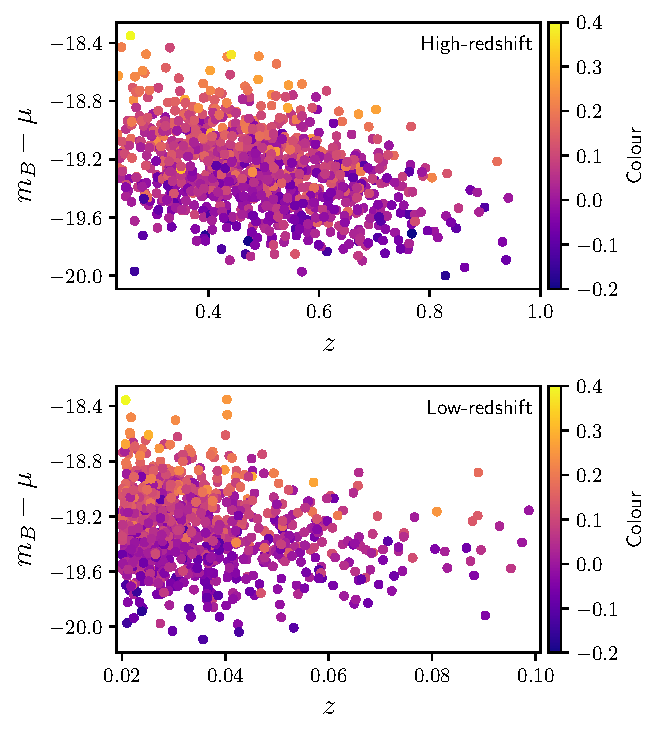
\includegraphics[width=\columnwidth]{plot_pop_simple.pdf}
	\end{center}
	\caption{Population distributions shown in redshift and uncorrected absolute magnitude $m_B - \mu$ for 1000 supernovae in both high-redshift and low-redshift surveys. Selection effects are visible in both samples, where red supernovae are often cut as redshift increases.}
	\label{fig:simple_pop}
\end{figure}
\begin{figure}
	\begin{center}
		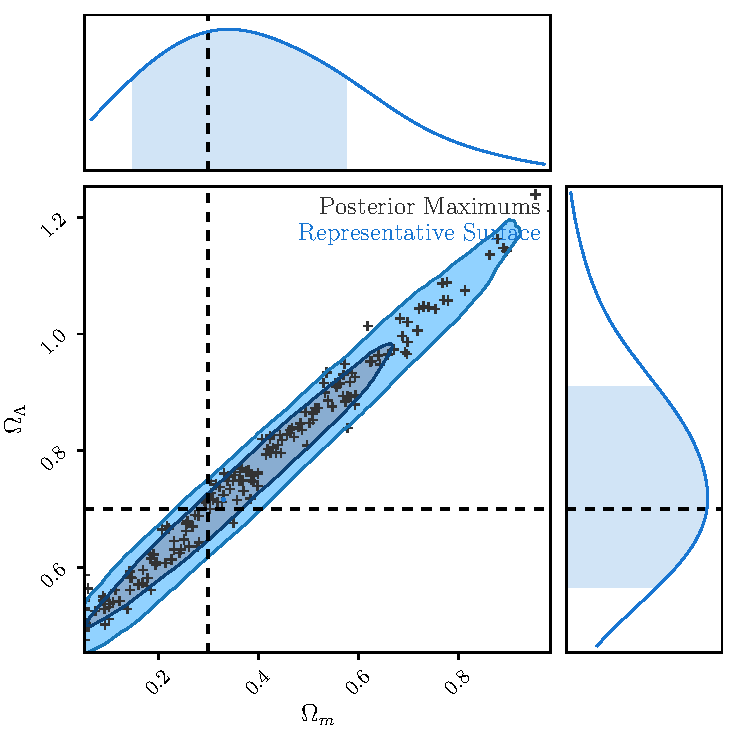
\includegraphics[width=\columnwidth]{simpleApproximateModelOl.pdf}
	\end{center}
	\caption{Posterior surfaces for 100 realisations of supernova data with the $\Lambda$CDM model. Even a large supernova sample when treated robustly is insufficient to provide tight constraints on either $\Omega_m$ and $\Omega_\Lambda$ due to the severe degeneracy between the parameters.}
	\label{fig:simple_ol}
\end{figure}
\begin{figure}
	\begin{center}
		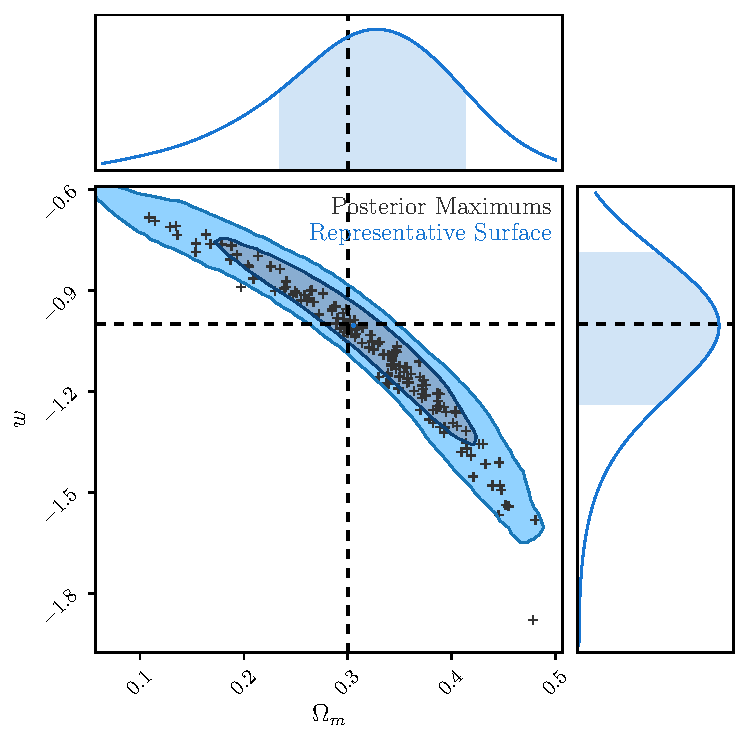
\includegraphics[width=\columnwidth]{simpleApproximateModelW.pdf}
	\end{center}
	\caption{Posterior surfaces for 100 realisations of supernova data with the Flat $w$CDM model. The well known banana shaped contour is recovered, with the marginalised distributions in $\Omega_m$ and $w$ providing incorrect statistics due to the highly non-Gaussian nature of the posterior surface.}
	\label{fig:simple_w}
\end{figure}

We generate simple toy data to validate the basic premise of the model. For both high-redshift and low-redshift (LowZ) data we draw from an underlying $M_B$, $x_1$, $c$ population and translate into apparent magnitude space using $\Omega_m = 0.3$, $\alpha= 0.14$ and $\beta = 3.1$. Masses are randomly drawn from the interval 0 to 1, and a mass correction with $\delta(0) = 0.08$ and $\delta(0)/\delta(\infty) =0.5$ included. Absolute magnitudes are drawn from $\mathcal{N}(-19.3, 0.1)$, true stretch values are drawn from $\mathcal{N}(0, 1)$ and true colour values are drawn from $\mathcal{N}^{\rm Skew}(0, 0.1, 2)$. Redshifts are drawn from a power law to increase the number of events as redshift increases. 

Independent observational errors of $0.04$, $0.2$, $0.03$ on $m_B$, $x_1$ and $c$ (following the mean uncertainty for DES SNANA simulations) are added to create the observables. Extra dispersion of $0.02(1+3z)$ is added in quadrature to the $c$ uncertainty to simulation unexplained colour dispersion from chromatic variation in supernovae. The selection functions (a skew normal for low-redshift and an error function for high-redshift) are given independent uncertainty of $0.01$ on all parameters. The results are then passed through the selection effects, where each supernova is only selected based on $P(S|m_B)$, using a skew normal function for the LowZ supernovae and error function for the DES-like supernovae. We draw from each survey simulation until we have 1000 LowZ supernovae and 1000 DES-like supernovae, representing a statistical sample of greater power than the estimated 250 supernovae for the DES spectroscopic analysis. Sample data for 1000 high and low redshift supernovae are shown in Figure \ref{fig:simple_pop}, confirming the presence of strong selection effects in both toy surveys. 

We test four models: Flat $\Lambda$CDM, Flat $w$CDM, $\Lambda$CDM and Flat $w$CDM with a prior $\Omega_m \sim \mathcal{N}(0.3, 0.01)$, with the latter included to allow sensitive tests on bias for $w$. To achieve statistical precision, we fit 100 realisations of supernovae datasets. Cosmological parameters are recovered without significant bias. Combined posterior surfaces of all 100 realisations for Flat $wCDM$ fits are shown in Figure \ref{fig:simple_w}. By utilising the Stan framework and several efficient parametrisations (discussed further in Appendix \ref{app:optimisations}), fits to these simulations of 2000 supernovae take only on order of a single CPU-hour to run.

To enforce investigate biases in the model in fine detail, we look for systematic bias in $\Omega_m$ in the Flat $\Lambda$CDM cosmology test, and bias in $w$ for the Flat $w$CDM test with strong prior $\Omega_m \sim \mathcal{N}(0.3, 0.01)$. This allows us to investigate biases without the investigative hindrances of non-Gaussian or truncated posterior surfaces, and the results of the analysis are detailed in Table \ref{tab:simple_model}, and do not reveal evidence of systematic bias in our model.

\begin{table}
	\centering
	\caption{Maximum likelihood cosmological parameters determined from stacking the surfaces of 100 fits to independent realisations of toy supernova data. As described in the main text, each dataset comprised 1000 low-redshift supernovae and 1000 high-redshift supernovae. Model bias would appear as shifts away from the simulation values of $\Omega_m = 0.3$, $w = -1$. As our surfaces are stacked, a shift away from the simulated values of more than $\sigma/\sqrt{100} = 0.1\sigma$ would give a $1\sigma$ detection of bias. No significant bias is detected in either cosmological model.}
	\label{tab:simple_model}
	\begin{tabular}{l|cc}
		\hline
		Model & $\Omega_m$ & $w$ \\ 
		\hline
		Flat $\Lambda$CDM & $0.301\pm 0.016$ & -- \\ 
		Flat $w$CDM + $\Omega_m$ prior & $\left( 300.5^{+10.5}_{-9.8} \right) \times 10^{-3}$ & $-0.998^{+0.043}_{-0.047}$ \\ 
		\hline
	\end{tabular}
\end{table}




















\subsection{DES SN data validation}
\label{sec:simdes}


Early analyses often treated intrinsic dispersion simply as scatter in the underlying absolute magnitude of the underlying population, but recent analyses require more a more sophisticated approach. In our development of this model and tests of intrinsic dispersion, we analyse the effects of two different scatter models. The first model is the \citet[][hereafter denoted the {\gten} scatter model]{Guy2010}, which models intrinsic scatter with a 70\% contribution from coherent variation and 30\% from chromatic variation. The second model, denoted the {\celeven} model is sourced from \citet{Chotard2011} and has variation with 25\% contribution from coherent scatter and 75\% from chromatic variation. 

Simulations (using the SNANA package) follow the observational schedule and observing conditions for the DES and LowZ surveys. In addition to the improvements in the scatter models over the simple data, we also include peculiar velocities for the LowZ sample, and now also include our full treatment of systematics. Our simulated populations are sourced from \citet[][hereafter {\sk}]{Scolnic2016}. The selection effects observed by comparing the generated supernovae to those that pass our simulated cuts and were successfully `observed' are shown in Figure~\ref{fig:sf_snana}, and it is from this simulation that our analytic determination of the selection functions for the LowZ and DES survey are based. We note that there was no significant difference between using the {\gten} or {\celeven} scatter model compared to the fit uncertainty.


\begin{table}
	\centering
	\caption{Tested population distributions, where the {\sk} LowZ stretch distribution is formed as sum of two bifurcated Gaussians, with the mean and spread of each component given respectively.}
	\label{tab:dist}
	\begin{tabular}{l|cccc}
		\hline
		Model & $\langle x_1 \rangle$ & $\sigma_{x_1}$ &  $\langle c \rangle$ & $\sigma_c$  \\
		\hline
		{\sk} LowZ    &  $0.55$ \& $-1.5$ & $^{+0.45}_{-1.0}$ \& $^{+0.5}_{-0.5}$ & $-0.055$ & $^{+0.15}_{-0.023}$ \\
		{\sk} DES     & $0.973$ & $^{+0.222}_{1.472}$ & $-0.054$  &  $^{+0.101}_{0.043}$ \\
		\hline
	\end{tabular}
\end{table}




\begin{figure}
	\begin{center}
		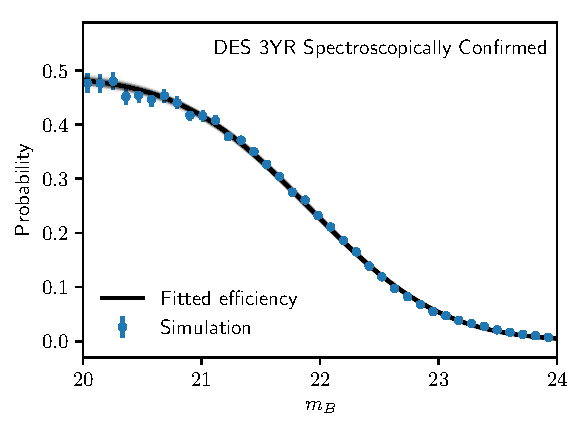
\includegraphics[width=\columnwidth]{DES3YR_DES_BHMEFF_AMG10.pdf}
		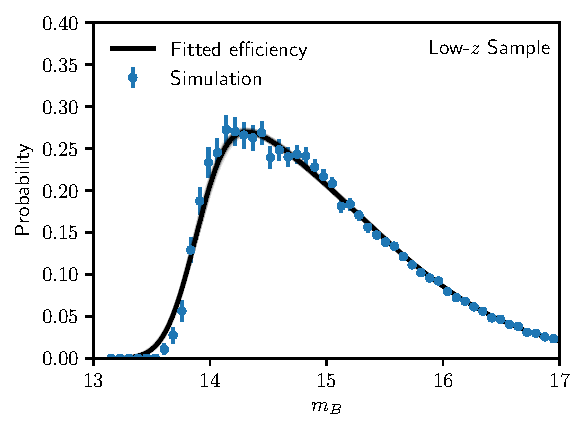
\includegraphics[width=\columnwidth]{DES3YR_LOWZ_BHMEFF_G10.pdf}
	\end{center}
	\caption{Fitting the selection function for both the DES 3YR spectroscopically confirmed supernova sample and the combined low-redshift sample. Blue errorbars represent the efficiency calculated by determining the ratio of discovered to generated supernovae in apparent magnitude bins for SNANA simulations. The black line represents the best fit analytic function for each sample, and the light grey lines surrounding the best fit value represent random realisations of analytic function taking into account uncertainty on the best fit value.}
	\label{fig:sf_snana}
\end{figure}








Each realisation of cosmology fitted contains 137 LowZ supernovae, and 204 DES-like supernovae, such that the uncertainties found when combining chains is representative of the uncertainty in the final DES spectroscopic analysis. As our primary focus is upon Dark Energy, we now focus specifically on the Flat $w$CDM model with matter prior.


 Combined posterior surfaces for 100 data realisations are shown in Figure \ref{fig:bulk_posterior}. Note that we have combined the posteriors for 100 realisations, and so we should expect the size of the uncertainty to be representative of one realisation, but the statistical spread of the final surface should be $\sqrt{100} = 10$ times less than a single realisation. The parameter bounds are listed in Table \ref{tab:bulk_summary}.
 
 
Cosmological bias is detected with $\approx 2.7\sigma$ significance for the {\celeven} model and $\approx 1.5\sigma$ significance for the {\gten} model when fitting both systematics and statistics. For the statistics only fits, the respective bias detection levels are $0.9\sigma$ and $5.5\sigma$. We investigate the source of the {\celeven} bias and find its source to be bias in the observed summary statistics, in addition to incorrect reported uncertainty on those summary statistics. By replacing fully simulated observed $m_B$, $x_1$ and $c$ with random numbers drawn from a true Gaussian centered on the simulated SALT2 $m_B$, $x_1$ and $c$ values with covariance as reported by initial light curve fits, both the {\gten} and {\celeven} fits recover $w=-1.00$ exactly. From this, the main challenge of improving our methodology is to handle the fact that observational uncertainty is incorrect, non-Gaussian and biased. Unfortunately, adding extra fit parameters to allow for shifting observables washes out cosmology, and applying a specific bias correction requires running a fiducial simulation (assuming cosmology, population and scatter model) and binning data, and is difficult to do whilst accounting for correlations with population and scatter model. This is compounded by the fact that bias corrections do not in general improve fits (increase the log posterior), and so are difficult to fit inherently. Colour bias corrections for the {\celeven} scatter model are included in our cosmology model, the strength of which are controlled by a fit parameter, $s_c$, however neither the {\gten} nor {\celeven} simulations constrained the fitting of this parameter, and thus the majority of bias in the {\celeven} fits remain. Works such as \citet{Kessler2017} show that bias corrections can be applied to supernovae datasets that can robustly handle multiple intrinsic scatter models, and future work will center on uniting these methodologies - incorporating better bias corrections without having to precompute standardisation parameters and populations.


For the sample size of the DES and LowZ supernova samples (of order 350 supernova), the bias from intrinsic scatter models are sub-dominant to the statistical uncertainty, representing at most a deviation of $0.27\sigma$ for the full statistics and systematics model fit for the {\celeven} model, and as such we will leave more complicated treatment of them for future work.

\begin{figure}
	\begin{center}
		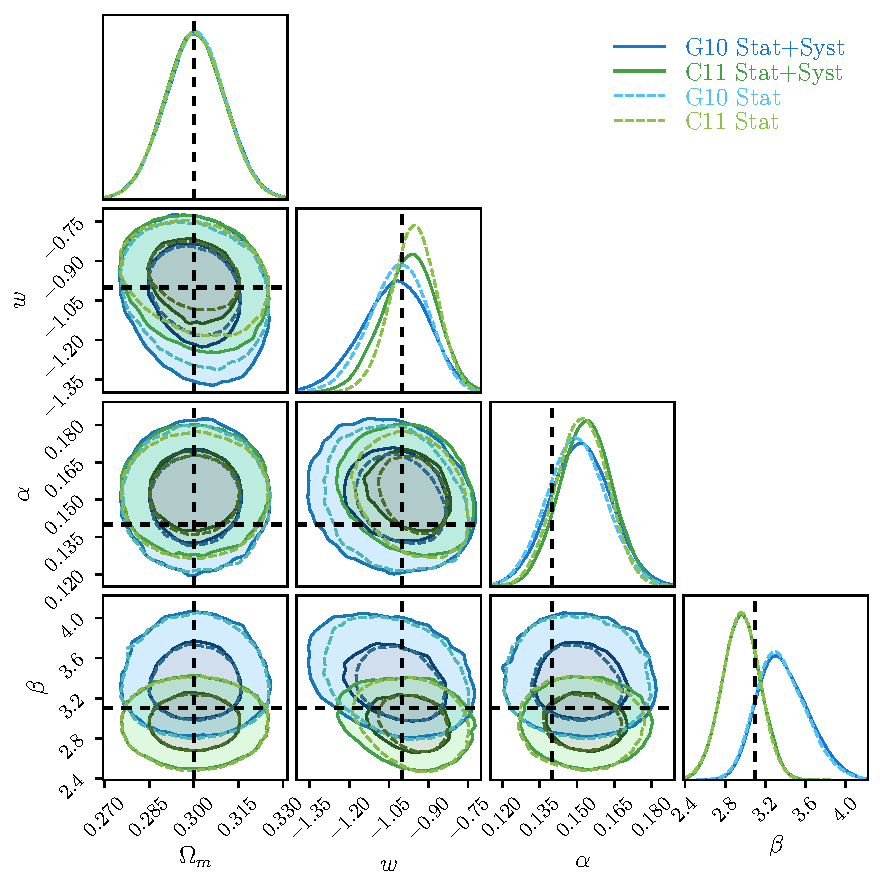
\includegraphics[width=\columnwidth]{bulk_small2.pdf}
	\end{center}
	\caption{Posterior surfaces for 100 realisations of supernova data. Surfaces for $\Omega_m$, $w$, $\alpha$, $\beta$ and $\langle M_B \rangle$ are shown, with the other fit parameters being marginalised over. The intrinsic scatter model has significant impact on the recovered $\beta$, which in itself effects cosmology, resulting in small biases in $w$.}
	\label{fig:bulk_posterior}
\end{figure}

\begin{table}
	\centering
	\caption{Investigating the combined 100 fits to {\gten} and {\celeven} simulations, fitting with both statistics only and also when including systematics. Whilst the {\gten} models do not show significant evidence of bias, the {\celeven} model does. With the current statistical size of the supernovae dataset, the bias is sub-dominant to the size of the uncertainty. }
	\label{tab:bulk_summary}
	\begin{tabular}{l|cc}
		\hline
		Model & $w$ & Bias Detection Level \\
		\hline
		{\gten} Stat + Syst  &  $-1.02\pm 0.13$ & $1.5\sigma$  \\
		{\celeven} Stat + Syst  &  $-0.97\pm 0.11$ & $2.7\sigma$  \\
		{\gten}  Stat         &  $-1.01\pm 0.11$ & $0.9\sigma$  \\
		{\celeven} Stat         &  $-0.95\pm 0.09$ & $5.5\sigma$  \\
		\hline
	\end{tabular}
\end{table}


\section{Conclusions}

In this paper we have outlined the creation of a Hierarchical Bayesian model for supernova cosmology. The model takes into account selection effects and their uncertainty, fits underlying populations and standardisation parameters, incorporates unexplained dispersion from intrinsic scatter colour smearing and incorporates uncertainty from peculiar velocity uncertainty, calibration uncertainty, dust uncertainty and SALT2 model uncertainty. The model has been optimised to allow for hundreds of supernovae to be modelled fully with latent parameters and run in under an hour of CPU time and scales linearly with the number of supernovae, as opposed to quadratic or cubic run times for models that rely on matrix inversion.

The importance of validating models using high-precision statistics gained by performing fits to hundreds of data realisations cannot be overstated, however is lacking in many prior BHM models for supernova cosmology. We have validated this model against many realisations of simplistic simulations with well-known and well-defined statistics, and found no bias. When validating using SNANA simulations, we find evidence of bias which is traced back to light curve fits reporting biased observables and incorrect covariance. Allowing fully parametrised corrections on observed supernovae summary statistics is found to make cosmology fits too weak, and allowing simulation based corrections to vary in strength is found to give minor reductions in bias, however the uncertainty on the intrinsic scatter model itself limits the efficacy of the bias corrections. For the data size represented in the DES three-year spectroscopic survey, the determined biases should be sub-dominant to other sources of uncertainty, however this cannot be expected for future analyses with larger datasets. Stricter bias corrections calculated from simulations are required to reduce bias. Ideally, this would include further work on the physical intrinsic dispersion of the Type Ia supernovae population such that we can better characterise this bias.

With our model being validated against hundreds of simulation realisations, representing a combined dataset over more than $250\,000$ simulated supernovae, we have been able to accurately determine biases in our model and trace their origin. With the current biases being sub-dominant to the total uncertainty, we now prepare to analyse the DES three-ear dataset. But that, my friends, is another, much more important, paper.

\section*{Acknowledgements}

Plots of posterior surfaces and parameter summaries were created with \verb|ChainConsumer| \citep{Hinton2016}.



%%%%%%%%%%%%%%%%%%%% REFERENCES %%%%%%%%%%%%%%%%%%

% The best way to enter references is to use BibTeX:

\bibliographystyle{mnras}
\bibliography{bib}




%%%%%%%%%%%%%%%%% APPENDICES %%%%%%%%%%%%%%%%%%%%%

\appendix

\section{Selection Effect Derivation}
\label{app:selection}

\subsection{General Selection Effects}

When formulating and fitting a model using a constraining dataset, we wish to resolve the posterior surface defined by
\begin{align}
P(\theta | {\rm data}) \propto P({\rm data} | \theta) P(\theta),
\end{align}
which gives the probability of the model parameter values ($\theta$) given the data.  Prior knowledge of the allowed values of the model parameters is encapsulated in the prior probability $P(\theta)$. Of primary interest to us is the likelihood of observing the data given our parametrised model, $\mathcal{L} \equiv P({\rm data} | \theta)$. When dealing with experiments which have imperfect selection efficiency, our likelihood must take that efficiency into account.  We need to describe the probability that the events we observe are both drawn from the distribution predicted by the underlying theoretical model \textit{and} that those events, given they happened, are subsequently successfully observed.  To make this extra conditional explicit, we write the likelihood of the data given an underlying model, $\theta$, \textit{and} that the data are included in our sample, denoted by $S$, as:
\begin{align}
\mathcal{L} &= P({\rm data} | \theta, S). \label{eq:app_like}
\end{align}
A variety of selection criteria are possible, and in our method we use our data in combination with the proposed model to determine the probability of particular selection criteria.  That is, we characterise a function $P(S|{\rm data},\theta)$, which colloquially can be stated as \textit{the probability of a potential observation passing selection cuts, given our observations and the underlying model}. We can introduce this expression in a few lines due to symmetry of joint probabilities and utilising that $P(x,y,z) = P(x|y,z)P(y,z) = P(y|x, z)P(x, z)$:
\begin{align}
P({\rm data} | S , \theta) P(S, \theta) &= P(S | {\rm data}, \theta) P({\rm data}, \theta)\\
P({\rm data} | S , \theta) &= \frac{ P(S | {\rm data}, \theta) P({\rm data}, \theta) }{ P(S, \theta) }\\
&= \frac{ P(S | {\rm data}, \theta) P({\rm data} | \theta) P(\theta)}{ P(S | \theta)  P(\theta)}\\
&= \frac{ P(S | {\rm data}, \theta) P({\rm data} | \theta)}{ P(S | \theta) }
\end{align}
which is equal to the likelihood $\mathcal{L}$. Introducing an integral over all possible events $D$, so we can evaluate $P(S|\theta)$, 
\begin{align}
\mathcal{L}&= \frac{P(S|{\rm data},\theta) P({\rm data}|\theta)}{\int P(S, D|\theta)\, dD} \\
\mathcal{L} &= \frac{P(S|{\rm data},\theta) P({\rm data}|\theta)}{\int P(S | D, \theta) P(D|\theta)\, dD}, \label{eq:app_main}
\end{align}
where we define the denominator as $w$ for simplicity in future derivations.



\subsection{Supernova Selection Effects}

We assume that our selection effects can be reasonably well encapsulated by independent functions of (actual) apparent magnitude and redshift, such that $P(S|{\rm data}, \theta) = P(S|z) P(S|m_B)$. Our denominator then becomes
\begin{align}
w &= \int d\hat{z} \, d\hat{m_B} \, dz \, dm_B P(S|z) P(S|m_B) P(\hat{z}|z) P(\hat{m_B}|m_B) P(z, m_B | \theta),
\end{align}
where for simplicity we have not written out all the integrals which do not interact with the selection effects explicitly. Due to our assumed perfect measurement of redshift, $P(\hat{z}|z) = \delta(\hat{z} - z)$. $P(\hat{m_B} | m_B)$ is a Gaussian due to our Gaussian model of summary statistics $m_B$, $x_1$, $c$, and can be analytically integrated out, collapsing the integral over $\hat{m_B}$. Finally, we can express $P(z, m_B | \theta)$ as  $P(m_B | z, \theta) P(z | \theta)$, where the first term requires us to calculate the magnitude distribution of our underlying population at a given redshift, and the second term is dependent on survey geometry and supernovae rates. We can thus state
\begin{align}
w = \int \left[ \int P(S|m_B) P(m_B | z, \theta)\, dm_B \right] P(S|z)P(z|\theta)\, dz.
\end{align}
By assuming that the distribution $P(S|z)P(z|\theta)$ is well sampled by the observed supernovae redshifts, we can approximate the integral over redshift by evaluating
\begin{align}
\int P(S|m_B) P(m_B | z, \theta)\, dm_B
\end{align}
for each supernova in the dataset -- i.e. Monte Carlo integration with assumed perfect importance sampling.

As stated in Section \ref{sec:selection}, the underlying population in apparent magnitude, when we discard skewness, can be represented as $\mathcal{N}(m_B|m_B^*(z), \sigma^*_{m_B})$, where
\begin{align}
m_B^*(z) &= \langle M_B \rangle + \mu(z) - \alpha \langle x_1(z) \rangle + \beta \left(\langle c(z) \rangle + \sqrt{\frac{2}{\pi}}\sigma_c \delta_c\right)\label{eq:disc1} \\
\sigma^*_{m_B} &= \sigma_{M_B}^2 + (\alpha \sigma_{x_1})^2 +  \left(\beta \sigma_c \sqrt{1 - \frac{2\delta_c^2}{\pi}}\right)^2. \label{eq:disc2}
\end{align}
Then, modelling $P(S|m_B)$ as either a normal or a skew normal, we can analytically perform the integral and reach equations \eqref{eq:seldes} and \eqref{eq:sellowz}.





\subsection{Approximate Selection Effects}
\label{app:approx}

Equations \eqref{eq:disc1} and \eqref{eq:disc2} make the assumption that, for our colour distribution, $\mathcal{N}^{\rm Skew}(\mu, \sigma, \alpha)$ is well approximated by $\mathcal{N}(\mu, \sigma)$. We sought to improve on this approximation by adjusting the mean and standard deviation of the approximated normal to match the actual mean and standard deviation of skew normal. With $\delta \equiv \alpha/\sqrt{1+\alpha^2}$, the correct mean and standard deviation are
\begin{align}
\mu_1 &= \mu_0 + \sqrt{\frac{2}{\pi}} \delta \sigma_0 \\
\sigma_1 &= \sigma_0 \sqrt{1 - \frac{2 \delta^2}{\pi}}.
\end{align}
We can then test the approximation $\mathcal{N}^{\rm Skew}(\mu_0, \sigma_0, \alpha) \rightarrow \mathcal{N}(\mu_1, \sigma_1)$. Unfortunately, this shift to the mean and standard deviation of the normal approximation did not produce stable posterior surfaces which Stan could fit when we included full covariance between $m_B$, $x_1$ and $c$ in the underlying population, and so we simplified the model to have independent parameters. Stable surfaces with underlying population covariance were found when we fixed $\sigma_c$ in the shift correction, such that $\mu_1 = \mu_0 + \sqrt{2/\pi}\delta k$, where we set $k=0.1$ to mirror the width of the input simulation population.  However, this resulted in several population parameters becoming biased, and so we do not fix $\sigma_c$. Comparing whether we shift our normal in the approximation or simply discard skewness, Figure \ref{fig:shift} shows that the calculated efficiency is significantly discrepant to the actual efficiency if the normal approximation is not shifted. The biases when using shifted or unshifted normal approximations when we fit our model on Gaussian and skewed underlying populations are shown in Figure \ref{fig:simple_w_super}, and only the shifted normal approximation correctly recovers underlying population parameters.

\begin{figure}
	\begin{center}
		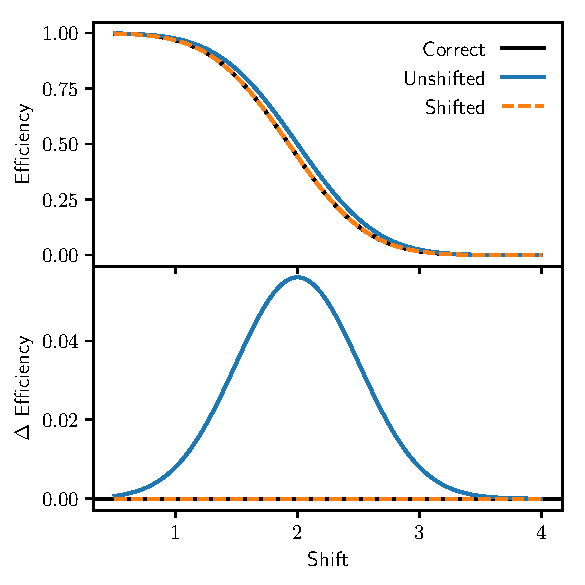
\includegraphics[width=\columnwidth]{shift.pdf}
	\end{center}
	\caption{Testing the correctness of our normal approximation to the skewed colour distribution. The `correct' line (shown in black) represents the exact integral $w = \int P(S|x) P(x) dx$ where $P(S|x)$ is an error function (following our high-redshift surveys) and $P(x) = \mathcal{N}^{\rm Skew}(x, 0.1, 2)$, calculated numerically. The $x$-axis is analogous to $m_B$ is cosmological context. As expected, all efficiencies drop towards zero as shift increases (as objects get fainter). The unshifted normal approximation shows significant discrepancy in the calculated efficiency as it transitions from 1 to 0, whilst the shifted normal approximation shows negligible error to the correct solution. From these plots, further refinement of the normal approximation (such as including kurtosis or higher powers) as unnecessary.}
	\label{fig:shift}
\end{figure}

\begin{figure*}
	\begin{center}
		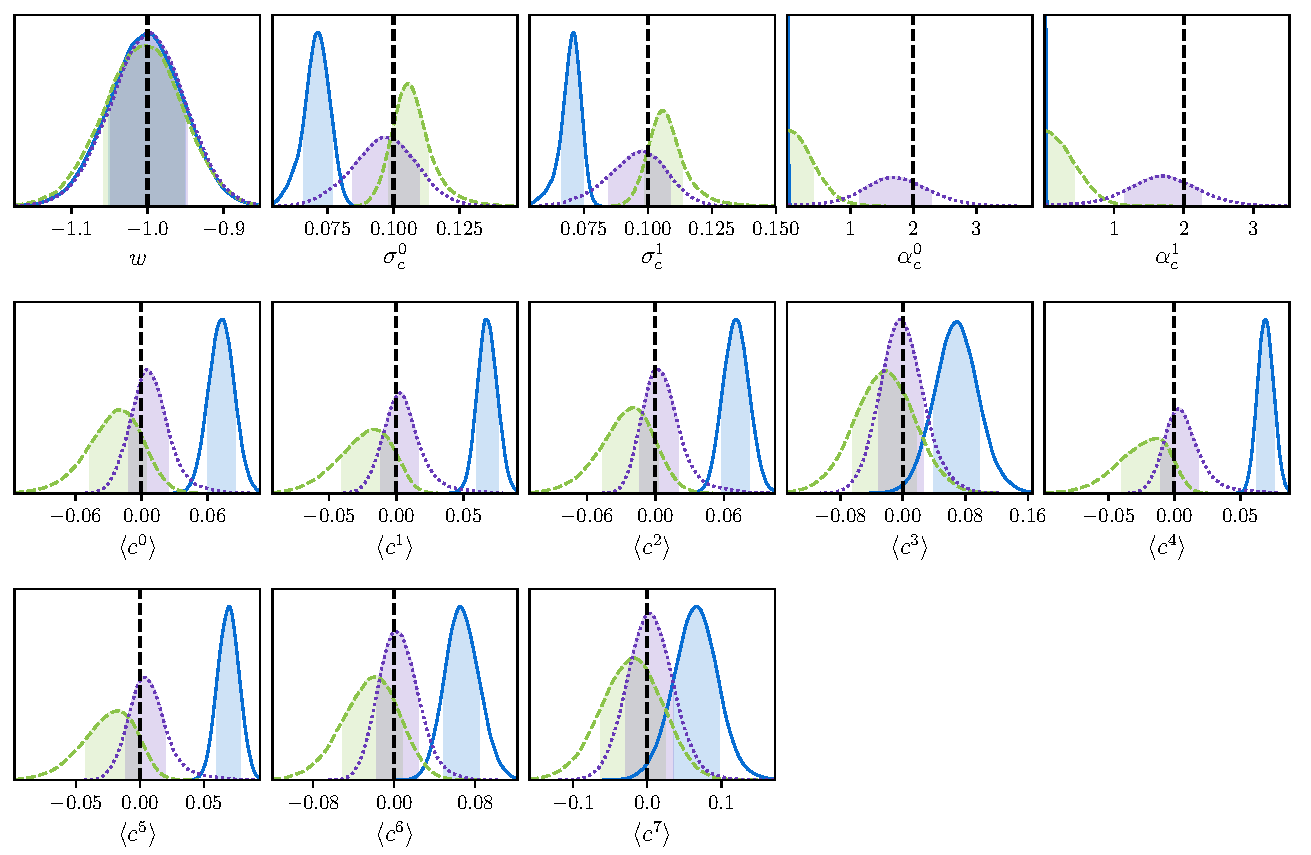
\includegraphics[width=\textwidth]{simple_w_shift_dist_0.pdf}
	\end{center}
	\caption{Marginalised probability distributions for 100 realisations of cosmology, fit to Flat $w$CDM with prior $\Omega_m \sim \mathcal{N}(0.3, 0.01)$, each containing 1000 simulated high-z and 1000 simulated low-z supernovae. The dashed green surfaces represent a fit to an underlying Gaussian colour population with the unshifted model. The blue solid surface represents fits to a skewed colour population with the unshifted model, and the purple dotted surface represents a fit to a skewed colour population with the shifted model. The superscript $0$ and $1$ denote the two different surveys (high-z and low-z respectively), and similarly the first four $\langle c^i \rangle$ parameters represent the four redshift nodes in the high-z survey, and the last four represent the nodes for the low-z survey. We can see that the shifted model is far better able to recover skewed input populations than the unshifted, performing better in terms of recovering skewness $\alpha_c$, mean colour $\langle c \rangle$ and width of the colour distribution $\sigma_c$. The unshifted model recovers the correct colour mean and width if you approximate a skew normal as a normal: $\Delta\mu = \sqrt{2/\pi}\sigma_c\delta_c \approx 0.071$, which is approximately the deviation found in fits to the colour population mean. Importantly, the unshifted model when run on skewed data (the solid blue) shows extreme bias in $\alpha_c$, where it fits strongly around zero regardless, showing it to be a poor approximation.}
	\label{fig:simple_w_super}
\end{figure*}


















\section{Numerical Optimisations}
\label{app:optimisations}


Not many fitting methodologies and algorithms can handle the thousands of fit parameters our model requires. By using Stan, we are able to take advantage automatic differentiation and the NUTS sampler, which is a class of Hamiltonian Monte Carlo samplers. Even with these advantages, early implementations of our model still had excessive fit times, with our desired sub-hour running time far exceeded. 

The simplest and most commonly found optimisation we employed was to precompute as much as possible to reduce the complexity of the mathematical graph our model is translated into to compute the surface derivatives. For example, when computing the distance modulus, redshift is encountered to various powers. Instead of computing those powers in Stan, we simply pass in several arrays of redshift values already raised to the correct power. Small changes like this however only give small results.

The primary numerical improvement we made on existing frameworks was to remove costly probability evaluations of multivariate normals. To increase efficiency, the optimum way to sample a multivariate normal is to reparameterise it such that instead of sampling $\mathcal{N}(\vec{x}|\vec{\mu}, \Sigma)$, you sample $\mathcal{N}(\vec{\delta}|0,1)$ where $\vec{x} = \vec{\mu} + L \vec{\delta}$ and $L$ is the cholesky decomposition of $\Sigma$. In this way, we can efficiently sample the unit normal probability distribution instead of sampling a multivariate normal probability distribution. Switching to this parametrisation resulted in a computational increase of an order of magnitude, taking fits for a sample of approximately 500 supernovae from roughly four hours down to thirty minutes. 

This parametrisation does come with one significant downside - inflexibility. For each step the algorithm takes, we do not recompute the cholesky decomposition of the covariance of the summary statistics - that happens once at the beginning of the model setup. If we had kept the full covariance matrix parametrisation we could modify the matrix easily - for example when incorporating intrinsic dispersion we could simple add on a secondary matrix to create an updated covariance. Using cholesky decompositions, ${\rm cholesky}(\Sigma_1 + \Sigma_2) \neq L_1 + L_2$, and so we would need to recompute the decomposition for each step, which discards most of the computational benefit just gained.

Considering a $3\times3$ matrix with cholesky decomposition
\begin{align}
L = \begin{pmatrix}
a & 0 & 0 \\ b & c & 0 \\ d & e & f \\
\end{pmatrix},
\end{align}
the original covariance matrix $\Sigma$ is given by
\begin{align}
\Sigma = \begin{pmatrix}
a^2 & ab & ad \\ ab & b^2 + c^2 & bd + ce \\ ad & bd + ce & d^2 + e^2 + f^2\\
\end{pmatrix}.
\end{align}
Now, the primary source of extra uncertainty in the intrinsic dispersion models comes from chromatic smearing, which primarily influences the recovered colour parameter, which is placed as the last element in the observables vector $\lbrace m_B, x_1, c\rbrace$. We can now see that it is possible to add extra uncertainty to the colour observation on the diagonal without having to recompute the cholesky decomposition - notice that $f$ is unique in that it is the only element of $L$ that appears in only one position in the covariance matrix. To take our covariance and add on the diagonal uncertainty for colour an extra $\sigma_e$ term, we get
\begin{align}
C = \begin{pmatrix}
\sigma_{m_B}^2 & \rho_{0,1} \sigma_{m_B} \sigma_{x_1} & \rho_{0,2} \sigma_{m_B} \sigma_c \\
\rho_{0,1} \sigma_{m_B} \sigma_{x_1} & \sigma_{x_1}^2 & \rho_{1, 2} \sigma_{x_1} \sigma_c \\
\rho_{0,2} \sigma_{m_B} \sigma_c & \rho_{1, 2} \sigma_{x_1} \sigma_c &  \sigma_c^2 + \sigma_e^2 \\
\end{pmatrix}
\end{align}.
The cholesky decomposition of this is, in terms of the original cholesky decomposition, is
\begin{align}
L = \begin{pmatrix}
a & 0 & 0 \\ b & c & 0 \\ d & e & f + g \\
\end{pmatrix},
\end{align}
where $g = \sqrt{f^2 + \sigma_e^2} - f$. This allows an easy update to the cholesky decomposition to add extra uncertainty to the independent colour uncertainty. For both the {\gten} and {\celeven} models, we ran fits without the cholesky parametrisation to allow for extra correlated dispersion (instead of just dispersion on $c$), but find no decrease in bias or improved fit statistics, allowing us to use the more efficient cholesky parametrisation.





% Don't change these lines
\bsp	% typesetting comment
\label{lastpage}
\end{document}

% End of mnras_template.tex